\section{Experimental Setup}


% \subsection{Wearable Thermal Data Collection Platform}
% \label{subsec:platform}

% It consists of three ultra-low-resolution thermal cameras, a synchronized RGB camera, and an embedded acquisition unit. 
% Our wearable platform (Fig.~\ref{fig:pipeline}) is designed around four goals: ultra-low unit cost,
% privacy-preserving sensing, portability, and label-free thermal supervision.
% Low unit cost keeps the platform plausible as an everyday aid. Privacy is
% preserved because the deployed device perceives its surroundings only through
% low-resolution thermal arrays~\cite{tao2018home,tateno2020privacy}.
% Portability ensures that the collected data reflect natural egocentric views
% rather than laboratory conditions. Label-free supervision draws navigability
% labels from a co-recorded reference view instead of hand annotation.

\subsection{Wearable Platform}
\label{subsec:platform}
The wearable platform (Fig.~\ref{fig:pipeline}) consists of an NVIDIA Jetson
Nano, three Melexis MLX90640 thermal cameras arranged in a forward-facing fan,
and a co-mounted Raspberry Pi Camera v2 used only to generate labels. The
thermal cameras provide left, middle, and right views, each a $32\times24$
image at 4\,Hz. The platform is built from commodity components for about
\$471, well below comparable wearable depth-based navigation
systems~\cite{li2025rgbd,bai2019wearable}. Thermal and RGB streams are
timestamped during acquisition and synchronized offline, discarding poorly
aligned samples before training.

% A person registers on
% the camera that faces them, while the other views remain near ambient
% temperature~\cite{newaz2024low,dubail2023privacy,papagianopoulos2023obstacle}.
% Each factory-calibrated camera returns a $32\times24$ array of absolute
% temperatures at 4\,Hz.
% Because the MLX90640 exposes a single fixed
% I\textsuperscript{2}C address, a TCA9548A multiplexer selects one camera
% per transaction.

% \paragraph{RGB supervision camera}
% A Raspberry Pi Camera v2 is rigidly mounted to the top of the thermal housing,
% with its optical axis aligned to the central thermal camera, recording
% $1280\times720$ JPEG frames at 4\,fps. It serves as a training-time supervisory
% instrument only and is not part of the deployed inference pipeline. Its
% high-resolution visible-light view provides the navigability labels for the
% co-recorded thermal frames during training, which avoids hand-annotating the
% low-resolution thermal data~\cite{devaguptapu2019borrow}.

% \paragraph{Packaging and software}
% A USB power bank keeps the unit untethered, and a 3D-printed housing fixes the
% three thermal cameras on a curved front face, with a separate printed case for
% the Jetson. The platform is built from low-cost commodity modules rather than
% the depth cameras used in comparable wearable navigation
% aids~\cite{li2025rgbd,bai2019wearable}, and costs approximately \$471 in
% parts. An on-board service starts and stops all sensors jointly and serves a
% live preview for in-field verification, with each sensor driven by an
% independent capture process so that a single-sensor fault cannot interrupt the
% remaining streams. Every sample is stamped at capture with a
% millisecond-resolution Unix timestamp from the shared system clock, which
% allows frames to be aligned in post-processing without hardware triggering.
% After each recording, the service maps every frame of the slowest stream to
% the temporally nearest frame of each remaining stream, retaining the residual
% offset so that poorly synchronized pairs can be discarded before training.
\subsection{Data Collection}
The dataset\footnote{The thermal frames, labels, and thermal homographies are available at \url{https://huggingface.co/datasets/Faiz3005/TartanThermals_Navigability_Dataset}, and the code at \url{https://github.com/jana-hussien/ershad}. RGB frames are withheld to protect the privacy of recorded individuals.} was collected on
the Carnegie Mellon University in Qatar (CMU-Q) campus and spans a variety of
indoor and outdoor scenes, planned to cover a free, a partially obstructed,
and a fully obstructed path (Table~\ref{tab:environments}); the per-direction
labels themselves come from the detector. A human operator wore
the platform and walked through each environment at a natural pace. Sessions were recorded
both with and without other people present, so that the automatic labeler
encountered a realistic mixture of \textit{clear}, \textit{person}, and
\textit{other-object} events. In total, the platform recorded about 116 minutes of data. The
experiments use 15,868 frames from 12 sessions, split at random into 12,697 for training and 3,171
for validation; a separate session of 988 frames, never used for training
or validation, is held out as the test set for the camera-arrangement
experiments. Fig.~\ref{fig:class_dist} shows the resulting class
distribution.
\begin{figure}[t!]
\begin{center}
\centering
\noindent
$\vcenter{\hbox{%
\begin{minipage}{0.42\linewidth}
\centering
\captionof{table}{Scene types encountered during data collection.}
\label{tab:environments}
\scriptsize
\renewcommand{\arraystretch}{1.0}
\setlength{\tabcolsep}{3pt}
% X column takes whatever width State/People leave, so nothing overlaps in any font
\begin{tabularx}{\linewidth}{@{}>{\raggedright\arraybackslash}Xll@{}}
\toprule
\textbf{Environment} & \textbf{Path} & \textbf{People} \\
\midrule
Open corridors              & Free    & No  \\
Stairwells                  & Free    & No  \\
Covered walkways            & Free    & No  \\
\midrule
Doorways                    & Partial & No  \\
Furniture in~path           & Partial & No  \\
Corridor with bystander     & Partial & Yes \\
\midrule
Crowded~lobbies              & Full    & Yes \\
Waiting~areas                & Full    & Yes \\
Building~entrances           & Full    & Yes \\
\bottomrule
\end{tabularx}
\end{minipage}%
}}$%
\hfill
$\vcenter{\hbox{%
\begin{minipage}{0.53\linewidth}
\centering
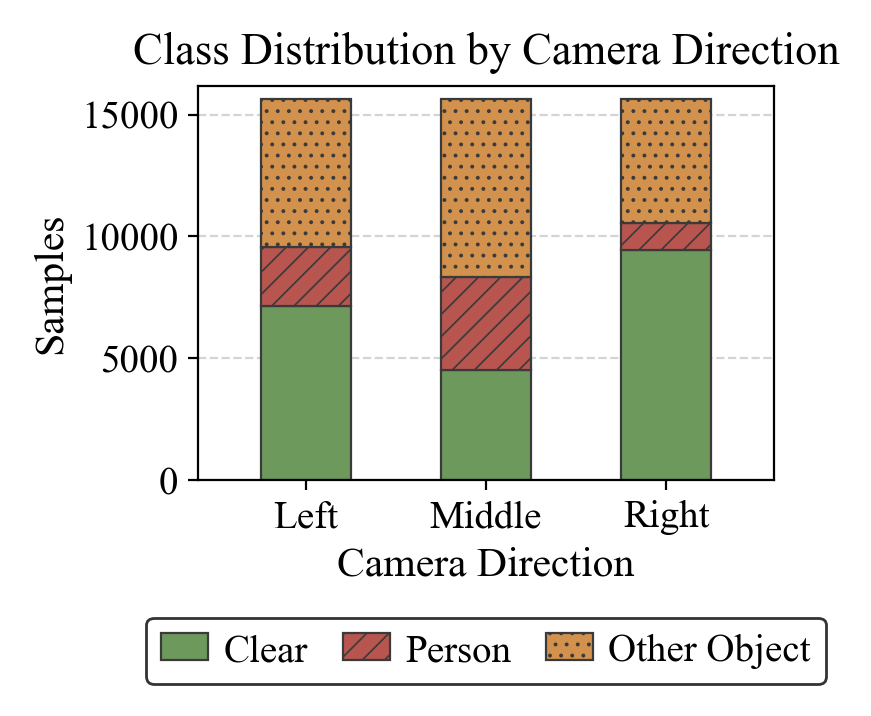
\includegraphics[width=\linewidth]{figs/fig3_new.png}
% 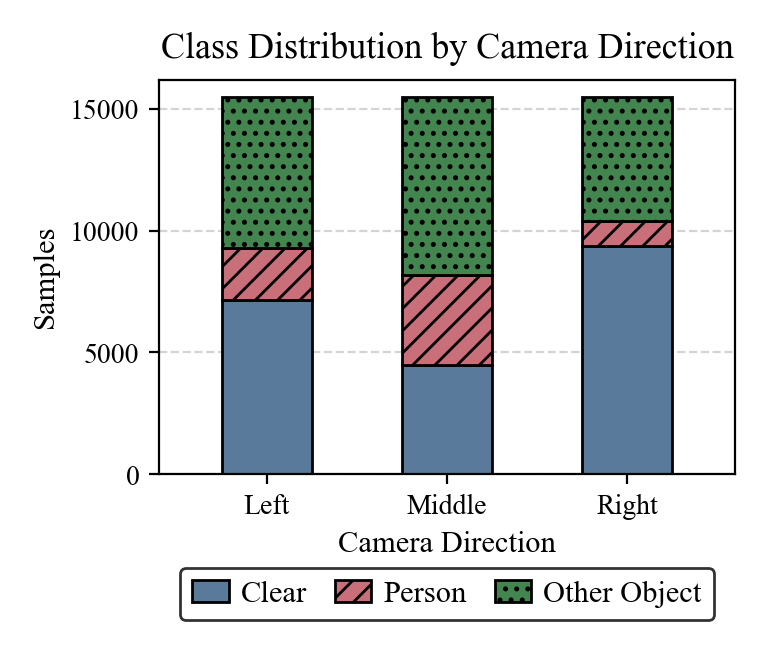
\includegraphics[width=\linewidth]{figs/fig3.png}   % previous version (counts estimated from an image)
\captionof{figure}{Class distribution across camera directions for the combined
training and validation split.}
\label{fig:class_dist}
\end{minipage}%
}}$

\end{center}
\end{figure}